\documentclass[tikz,border=5pt]{standalone}
\usepackage{amsmath}
\definecolor{curveblue}{HTML}{245C86}
\begin{document}
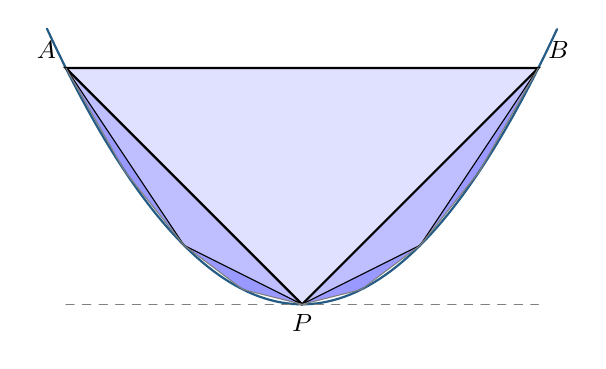
\begin{tikzpicture}[scale=3,font=\small,line cap=round]
\fill[blue!12](-1,1)--(0,0)--(1,1)--cycle;
\fill[blue!25](-1,1)--(-.5,.25)--(0,0)--cycle (0,0)--(.5,.25)--(1,1)--cycle;
\fill[blue!40](-1,1)--(-.75,.5625)--(-.5,.25)--cycle (-.5,.25)--(-.25,.0625)--(0,0)--cycle (0,0)--(.25,.0625)--(.5,.25)--cycle (.5,.25)--(.75,.5625)--(1,1)--cycle;
\draw[curveblue,thick,domain=-1.08:1.08,samples=90]plot(\x,{\x*\x});
\draw[thick](-1,1)--(1,1)--(0,0)--cycle;
\draw(-1,1)--(-.5,.25)--(0,0)--(.5,.25)--(1,1);
\draw[gray](-1,1)--(-.75,.5625)--(-.5,.25)--(-.25,.0625)--(0,0)--(.25,.0625)--(.5,.25)--(.75,.5625)--(1,1);
\node[above left]at(-1,1){$A$};\node[above right]at(1,1){$B$};\node[below]at(0,0){$P$};
\draw[gray,dashed](-1,0)--(1,0);
\end{tikzpicture}
\end{document}
